% Computer Architecture (4190.308) Fall 2016 
% Seoul National University CARES Lab
% Lab 4 documentation

% Lines that need modification : 27~29 (specific dates), 220~235 (results), 300~317 (results)
\documentclass{article}
\usepackage{graphicx, caption, subcaption, verbatim, moreverb, alltt, algorithm2e, kotex}
\usepackage[protrusion=true,expansion=true]{microtype}
\usepackage{fancyvrb}
\usepackage{hhline}
\usepackage{multirow}
\DeclareGraphicsExtensions{.pdf,.png,.jpg}
\let\verbatiminput=\verbatimtabinput

\setlength{\oddsidemargin}{0.25in}	% 1.25in left margin 
\setlength{\evensidemargin}{0.25in}	% 1.25in left margin (even pages)
\setlength{\topmargin}{0.0in}		% 1in top margin
\setlength{\textwidth}{6.0in}		% 6.0in text - 1.25in rt margin
\setlength{\textheight}{9in}		% Body ht for 1in margins
\addtolength{\topmargin}{-\headheight}	% No header, so compensate
\addtolength{\topmargin}{-\headsep}	% for header height and separation

\begin{document}

\title{Lab 6: 5-stage Pipelined Processor}   % type title between braces
\author{CSE 4190.308 Computer Architecture \\ 2 Exercises (Total 120 Points) }         
\date{Received: May , 2016 \\Due: 3:00 p.m., May , 2016\\ \ \\ TA Office Hours: 7:00 - 8:00 p.m., 5/, 5/, 5/}    % type date between braces
\maketitle

\section{Introduction}

In this lab, you will be given a 2-stage pipelined processor,
and change it into a 5-stage pipelined processor.
Because all kinds of hazards covered in class will exist in a 5 stage
pipeline, it will be your job to use methods such as epochs, scoreboards and bypassing (forwarding)
correctly to implement a functionally correct
and efficient 5-state pipelined processor.

%Compiling and running the code can be done identically to the previous
%labs, using the \texttt{y86} run script.

\section{Getting Started}
\subsection{How to Download the Source Code}
Lab 6의 실습 코드를 받기 위해 수업 홈페이지에 올라와 있는 \texttt{add-lab6.sh} 스크립트를 다운받고,
이전 Lab들을 수행했던 실습 디렉터리의 상위에 위치시킨 뒤 본인의 ID를 인자로 실행시킵니다.
archi16의 password(강의 홈페이지 비밀번호)와 본인의 svn 계정 비밀번호를 입력하면 실습 코드 다운이 완료됩니다.
실습 디렉터리 아래에 \texttt{lab6} 디렉터리가 새롭게 생성되었을 것입니다.

\begin{Verbatim}[frame=single]
   $ ./add-lab6.sh YOUR_ID

   archi16@hyewon.snu.ac.kr's password: 

   Password for 'YOUR_ID': 

   $ ls YOUR_ID/
   ... lab4/ lab5/ lab6/
\end{Verbatim}

\subsection{Directory Structure of Lab 6}
Lab 6 실습의 디렉터리 구조는 다음과 같습니다.

\begin{Verbatim}[frame=single]
lab6/
    src/	
        Proc.bsv
        y86
    lib/
        common-lib/
        programs/
        ...
\end{Verbatim}

\begin{description}
\item [\texttt{src/}]\hfill \ \\
	Lab 6 실습을 진행할 디렉터리입니다.

\item [\texttt{src/Proc.bsv}]\hfill \ \\
	2-stage pipeline Y86-64 프로세서가 구현되어 있는 파일입니다.

\item [\texttt{src/y86}]\hfill \ \\
	구현한 프로세서를 컴파일하고 벤치마크 프로그램을 실행할 수 있는 스크립트 파일입니다.

\item [\texttt{lib/}]\hfill \ \\
	Lab 에서 구현한 Y86-64 프로세서를 동작시키는 데 필요한 라이브러리 및 프로그램을 포함하고 있습니다.

\item [\texttt{lib/common-lib/}]\hfill \ \\
	프로세서를 구현할 때 사용되는 라이브러리 bsv 파일들입니다.

\item [\texttt{lib/programs/}]\hfill \ \\ 
	구현한 프로세서를 테스트하기 위한 벤치마크 프로그램들입니다.

\end{description}

\subsection{How to Simulate the Design}
Lab5에서와 같이 y86 스크립트를 통해 컴파일 및 벤치마크 프로그램 수행을 할 수 있습니다.
\subsubsection{Compiling and Simulation in Exercise}
 구현의 검증은 아래와 같이 \texttt{y86}
 스크립트를 실행하여 이뤄집니다. 
\begin{Verbatim}[frame=single]
    $ ./y86 -c 
    $ ./y86 -r
\end{Verbatim}
\noindent먼저, -c 플래그로 구현한 Y86-64프로세서를 컴파일을 할 수 있습니다.
다음, -r 플래그로 모든 벤치마크 수행을 테스트하거나, \texttt{-p} 플래그를 통해 특정 벤치마크 프로그램을 
테스트할 수 있습니다. 각 테스트가 끝나면, PASS 여부 및 수행한 사이클과 명령어 수가 출력됩니다.\\
y86 스크립트의 인자에 대한 자세한 내용은 다음과 같은 명령을 통해 확인하실 수 있습니다.
\
\begin{Verbatim}[frame=single]
./y86 -h
\end{Verbatim}

\subsubsection{Analyzing Simulation Result}
You can also see what happened in each pipeline step of each cycles.
You will find directories named as the benchmarks in the \texttt{Log} directory
after you finished running benchmark programs. The \texttt{simOut} files in these
directories contain the information on how instructions passed by each pipeline stages
while executing the corresponding benchmark. This may help your debugging.

\subsection{How to Submit Your Design}
Move into your \texttt{lab6/src} directory and type \texttt{svn commit} command.
Changed files will be uploaded to svn server.\\\\

\newpage
\section{A 5-stage pipeline}

The given 2-state pipeline has two rules, \texttt{doFetch} and
\texttt{doExecute} for fetch and execute rules. A 5-state pipelined
processor naturally needs 5 rules, for fetch, decode,
execute, memory read/write and register writeback.

Each stage of the pipeline have been implemented with a function, as
described in the table below.

\begin{table}[h]
\centering
\begin{tabular}{|c|c|}
\hline
Pipeline Stage & Function name \\
\hline
Fetch & iMem.req \\
Decode & decode/rf.rdA/rf.rdB \\
Execute & exec \\
Memory & dMem.req \\
Writeback & rf.wrE/rf.wrM \\
\hline
\end{tabular}
\end{table}

%The epoch scheme for dealing with control hazards are implemented
%similarly to previous labs, but you should consider that RET instruction obtains
%correct PC in Mem stage.

\subsection{FIFOs}

Bluespec에는 다음과 같은 특별한 종류의 FIFO들이 정의되어 있습니다. 
이번 lab에서는 이러한 FIFO들에 대한 이해를 바탕으로 오직 아래의 두 종류의 FIFO만 사용하셔야 합니다.
\\(주의사항 : 사용하는 모든 FIFO는 mkPipelineFifo 혹은 mkBypassFifo 중 하나로 초기화할 것. mkCFFifo는 사용 금지.)

%There are some special FIFOs you should know in order to perform this lab. 

\begin{itemize}
\item In a \textit{Pipeline FIFO}, we can \texttt{enq} and \texttt{deq} concurrently even
when it already contains a element, with the following logical ordering:
\\\\$\phantom{123123123123}$ first $<$ enq
\\$\phantom{123123123123}$ deq $<$ enq\\\\
This ordering makes it clear that the element returned by first is the element already
in the FIFO; that deq logically empties the FIFO; and that enq then inserts a new
element into the FIFO. When the FIFO is empty, first and deq are not enabled, and
there is no concurrency. The pipeline FIFO is implemented as \texttt{mkPipelineFifo}.

\item In a \textit{Bypass FIFO}, we can \texttt{enq} and \texttt{deq} concurrenty even when it contains no elements,
with the following logical ordering:
\\\\$\phantom{123123123123}$ enq $<$ first
\\$\phantom{123123123123}$ enq $<$ deq\\\\
This ordering makes it clear that enq inserts a new element into the empty FIFO,
and this is the element returned by first and emptied by deq. Thus, the enqueued
element can "fly through" the FIFO within the same clock, which is why it is called a
Bypass FIFO. When the FIFO is full, enq is not enabled, and there is no concurrency.
The bypass FIFO is implemented as \texttt{mkBypassFifo}.
\end{itemize}

Typically, Pipeline FIFOs are used in the forward direction of a pipeline, and
Bypass FIFOs are used for feedback paths that go upstream against the pipeline data flow.

\newpage
\subsection{Scoreboard}

In the pipelined processor, the register values to be fetched can be stale 
if they have been modified by some older instructions still in the pipeline.
This situation is referred to as a read-after-write(RAW) data hazard.
The \texttt{scoreboard} is a data structure to keep track of the instructions
in the pipeline beyond the fetch stage, and it is a easy solution to handle the RAW hazard.
By keeping the destination register of the last executed instruction, you can compare it
with the source registers of new instructions. The scoreboard is implemented
in \texttt{mkPipelineScoreboard}.

\begin{figure}[htbp]
	\begin{center}
		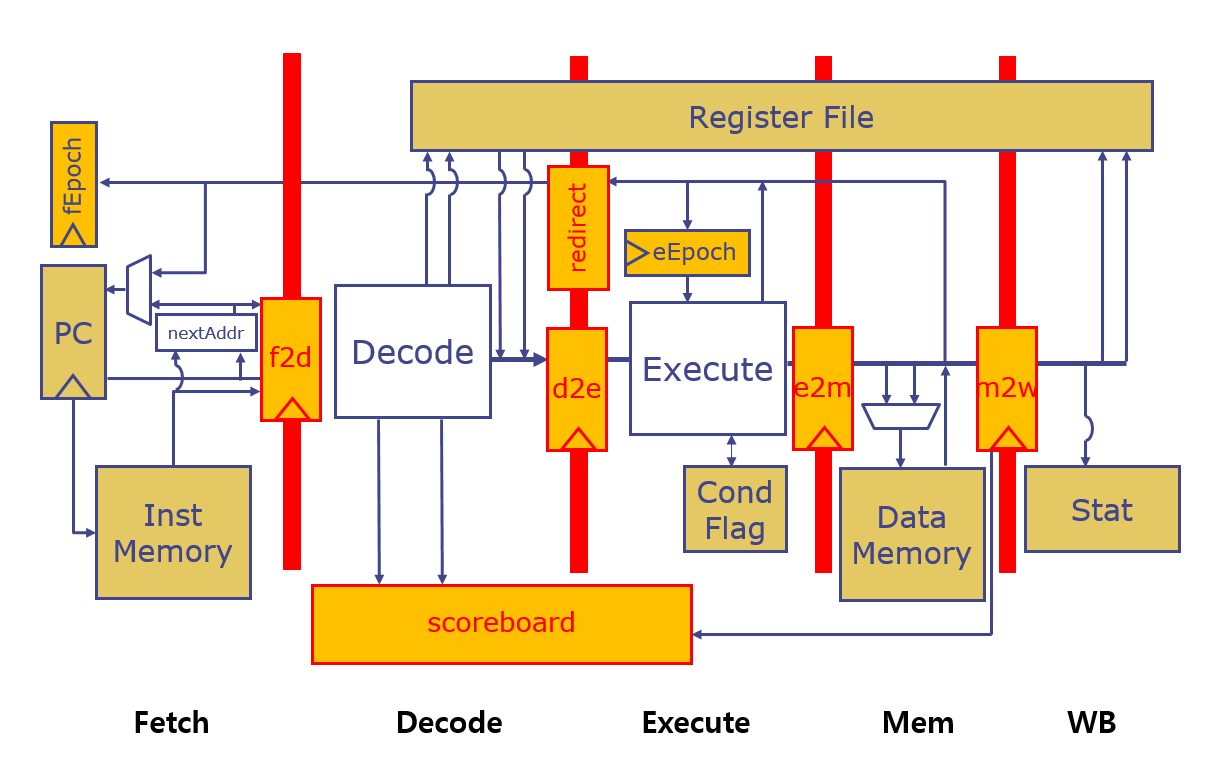
\includegraphics[scale=0.4]{5-stage.png}
		\caption{a 5-stage pipelined processor with a scoreboard}
		\label{fig:2pipe_proc}
	\end{center}
\end{figure}

\noindent \paragraph{\bf Exercise 1 (50 points) :} 첫 번째 문제는 기존의 2-stage pipelined processor를 
위에서 설명한 5-stage의 pipelined processor로 구현하는 것입니다. 이를 위해서는 각 stage 사이에 적절한 종류의 FIFO를 선택하고
추가적으로 epoch와 scoreboard 등을 이용하여 hazard를 처리하는 부분도 구현하셔야
합니다.\\
(Hint : 구현해야 할 pipeline의 stage 수가 5개로 늘어남에 따라 control hazard의
처리는 Execute stage 뿐만 아니라 Mem stage에서도 고려해야 합니다.)
%또한, miss prediction으로 인한 주소를 fetch 단계에서 bypassing으로 넘겨받는 상황에 대한 최적화(lab5의 \texttt{Exercise 1})도
%함께 고려하여 아래 표와 유사한 수준의 결과를 얻으셔야 합니다.

%Your job is to divide the two stages into the 
%six stages as above. You have to add an appropriate type of FIFOs (which have mentioned above) between them, 
%and adjust the application of the hazard dealing functionality (e.g. epoch, scoreboard) to ensure 
%correctness and efficiency.

\begin{table}[h]
\centering
\begin{tabular}{|c|c|c|c|}
\hline
Benchmark & Number of Instruction & Clock Cycles & IPC \\
\hline
median & 6871 & 14683 & 0.468\\
qsort & 21626 & 43675 & 0.495\\ 
multiply & 21098 & 51777 & 0.407\\
vvadd & 3018 & 4837 & 0.624\\
towers & 9907 & 17415  & 0.569\\
filters & 868217 & 2176898 & 0.399\\
\hline
\end{tabular}
\caption{Scoreboard를 사용한 5-stage pipelined processor의 실행 결과}
\end{table}

\newpage
\subsection{Bypassing (a.k.a forwarding)}

\texttt{Bypassing} is a more efficient method to solve the RAW hazard. All you can do by using
scoreboard is just to make a stall when the source register to be read is stale.
Meanwhile, in the bypassing method, the modified result is passed to earlier stage which needs
it in the same cylce. Therefore, the processor can operate normally without any cycle waste.

\begin{figure}[htbp]
	\begin{center}
		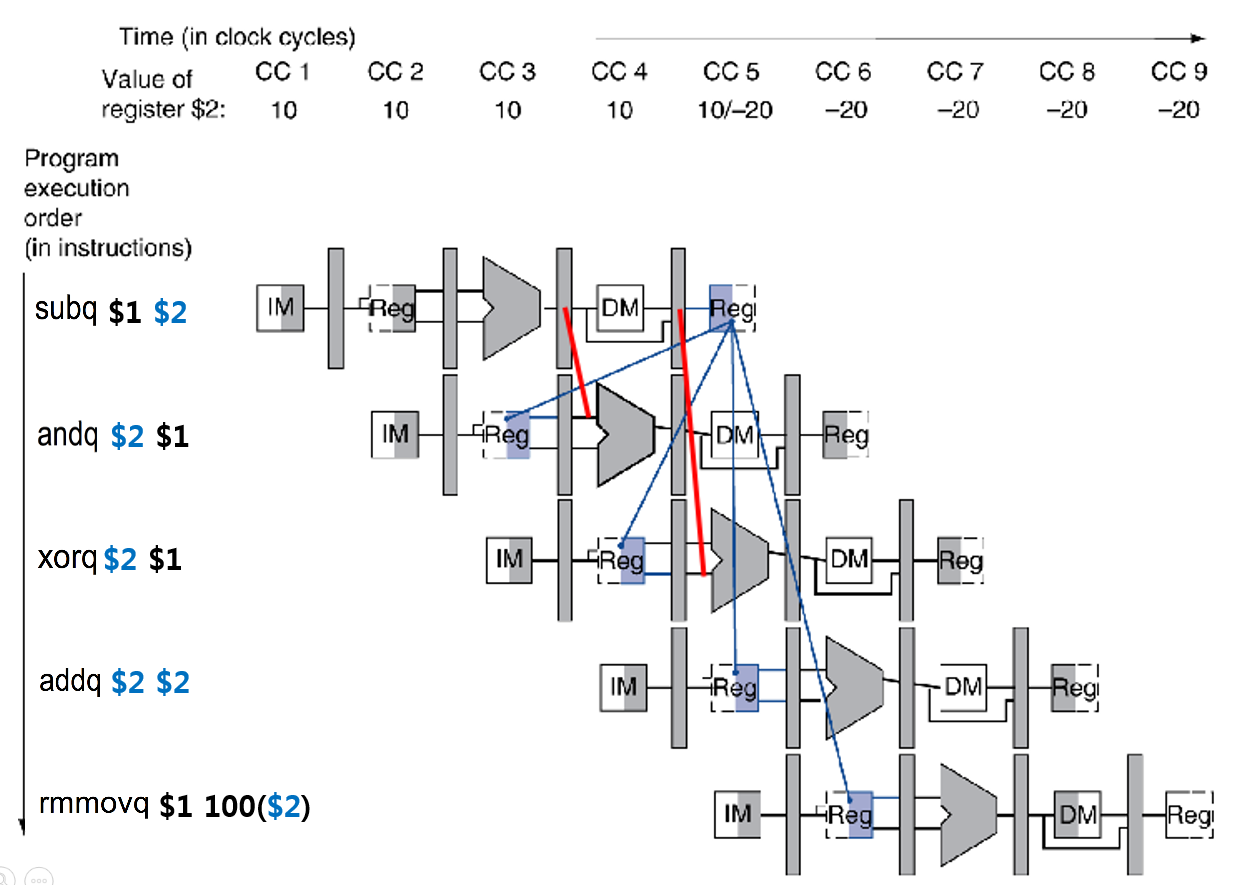
\includegraphics[scale=0.3]{forwarding.png}
		\caption{a bypassing example}
		\label{fig:2pipe_proc}
	\end{center}
\end{figure}

그러면 실제 5-stage pipelined processor에서 bypassing이 필요한 경우는 어떤 것들이 있는지 
살펴보도록 하겠습니다. 
\\
\begin{figure}[htbp]
	\begin{center}
		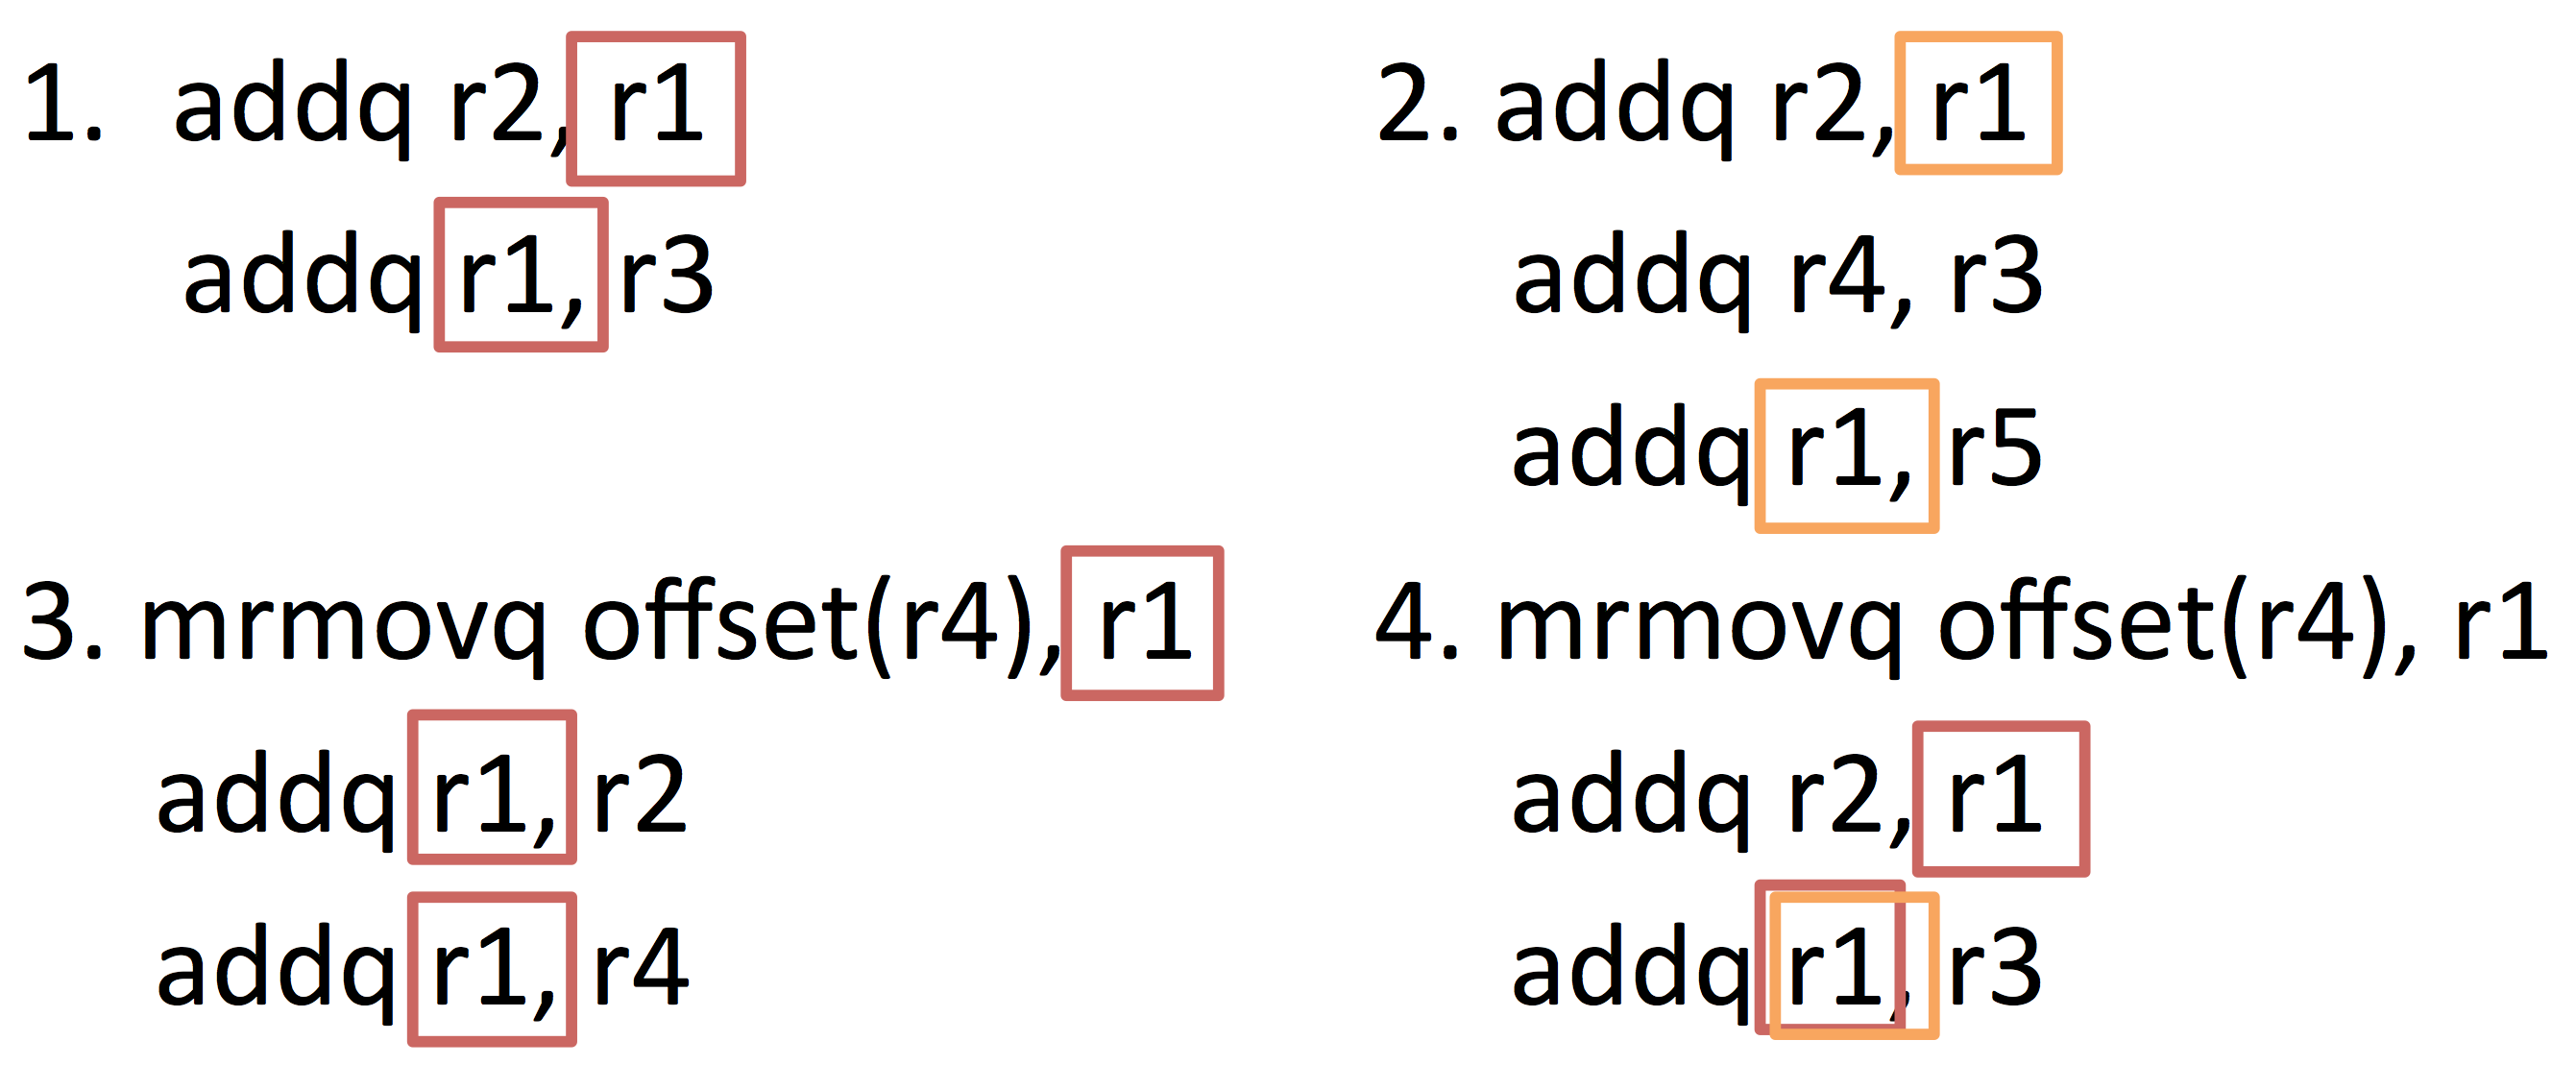
\includegraphics[scale=0.1]{ex.png}
		%\caption{아래 행일수록 최근에 실행된 Instruction}
		\label{fig:2pipe_proc}
	\end{center}
\end{figure}
%\begin{center}
%		아래 행일수록 최근에 실행된 Instruction
%\end{center}

\noindent 먼저, 1번의 상황은 현재 `Decode' stage에서 읽으려는 register가 바로
이전 instruction에 의해 변경된 경우입니다. (아래쪽 행일수록  최근에 실행된
instruction)
이전 instruction에 의해 r1의 값이 변경되었지만 아직 register에 변경된 값이 쓰이기 전이므로, 정상적인 수행을 위해서는 stall이나 
bypassing(`Execute'-$>$`Decode')이 필요하게 됩니다.\\
\\2번의 경우는 기본적으로 현재 `Decode' stage에서 읽으려는 register가 이전 instruction에 의해 변경되었으나 아직 register에
다시 쓰이기 전이라는 상황은 1번과 동일합니다. 하지만, bypassing을 해야하는 위치에 차이가 있습니다. 바로 전 instruction이 아닌 그보다 한 단계
이전의 instruction에 의해 register의 값이 변경되므로, 여기서는
`Memory'-$>$`Decode'로의 bypassing이 필요합니다.\\
\\한편, 3번의 경우는 Load instruction과 관련하여 발생할 수 있는 문제입니다. 이
경우 Load instruction가 `Memeory' stage에 있을 때, 
연이은 두 instruction을 위해 `Execute' stage와 `Decode' stage 두 곳에 모두 r1에 대한 bypassing을 해주어야 합니다.\\
\\마지막으로, 위와 같은 상황들을 해결하기 위해 bypassing을 구현하는 경우
4번에서와 같이 현재 수행하는 instruction의 `Decode'
stage에 총 2개의 bypassed data가 주어지게 됩니다. 이 때 어느 것이 더 최신의 값인지 선택하는 구현이 필요합니다.\\
\\
위에서 살펴본 것과 같이, 5-stage의 pipelined processor의 bypassing을 구현하기
위해서는 `Execute'-$>$`Decode'로 전달하는 것은 물론
`Memory'-$>$`Decode'와 `Memory'-$>$`Execute'로 전달하는 것까지 총 3가지를 고려해주어야 합니다.

\noindent \paragraph{\bf Exercise 2 (70 points) :} 두 번째 문제는 \texttt{Exercise 1}에서 구현한 5-stage pipelined processor를
보다 효율적인 형태로 개선하는 것입니다. 기존의 Scoreboard로 RAW hazard를 처리하는 방법 대신 Bypassing method를 사용하여
구현해주시면 됩니다. 단, 채점을 위해 \texttt{Exercise 2}는 기존의 'Proc.bsv'를 복사하여 'Proc\_bp.bsv'라는 파일을 만든 후,
'Proc\_bp.bsv'를 수정하는 방식으로 구현해주시기 바랍니다. 
\\(Proc.bsv : \texttt{Exercise 1},  Proc\_bp.bsv : \texttt{Exercise 2}) 
\\(주의 : 파일 복사 후 \texttt{\$ svn add Proc\_bp.bsv} 명령을 입력해야 제출시 Proc\_bp.bsv 파일도 함께 제출됩니다.)

%You have to implement 5-stage pipelined processor with \texttt{bypassing} method, not the \texttt{scoreboard}.
%Make a 'Proc\_bp.bsv' file by copying the 'Proc.bsv' after you have implemented the 5-stage pipelined processor 
%and then modify it for \texttt{Exercise 2}.
%\\Thus, you must have two modified files after you have finished this lab, 'Proc.bsv' for \texttt{Exercise 1} 
%and 'Proc\_bp.bsv' for \texttt{Exercise 2}.

\begin{table}[h]
\centering
\begin{tabular}{|c|c|c|c|}
\hline
Benchmark & Number of Instruction & Clock Cycles & IPC \\
\hline
median & 6871 & 9391 & 0.732\\
qsort & 21626 & 25432 & 0.850\\ 
multiply & 21098 & 33336 & 0.633\\
vvadd & 3018 & 3628 & 0.832\\
towers & 9907 & 12075 & 0.820\\
filters & 868217 & 1389923 & 0.625\\
\hline
\end{tabular}
\caption{Bypassing을 사용한 5-stage pipelined processor의 실행 결과}
\end{table}

\end{document}
